\section{A model of average road speed}
\label{sec:nw_model}


The relationship between the underlying road speed and the value observerd in \cref{cha:vehicle_model} involves two steps. First, we must describe the relationship between the average traffic speed and the vehicle's true average speed. Second, we define the relationship between \emph{actual} and \emph{observed} (or, more specifically, estimated) average speed. This type of model is referred to as a \emph{heirarchical (Bayesian) model} and was demonstrated graphically in \cref{fig:nw_model_hierarchy}.


Let us first consider the state of the network at time $t_c$, which we denote
\begin{equation}\label{eq:nw_state}
\boldsymbol{\NWstate}_c =
\left[\NWstate_{1,c}\ \cdots\ \NWstate_{L,c}\right]^\top,
\end{equation}
a vector containing the current real-time average traffic speed along all $L$ roads in the network. However, modelling the full state would increase computational demand as $L$ gets large, so we consider each road segment $\ell$ \emph{independently} (see later in \cref{sec:kf-limits} for a discussion of the implications of this).


Vehicles travelling along road segment $\ell$ at time $t_c$ have an underlying average speed of $\NWstate_{\ellc}$~seconds, which changes with an average rate of $\NWnoise_\ell$. Assuming the underlying road state is a Markov process, the model for the evolution of traffic speed along a road with a maximum velocity (speed) of $\MaxSpeed_\ell$~\gls{mps} is
\begin{equation}\label{eq:nw_state_markov}
\NWstate_{\ellc} \sim
\TNormal{\mathcal{F}_c(\NWstate_{\ellc-1})}{(\NWtdiff_c \NWnoise_c)^2}{0}{\MaxSpeed_\ell}
\end{equation}
where $\NWtdiff_c = t_c - t_{c-1}$ is the time since the last update. This model allows traffic speed to follow temporal trends through the time-dependent transition matrix $\mathcal{F}_c$ (peak hour traffic, for example) as well as react to real-time events, such as accidents or weather events


As already mentioned, there are many factors which can affect the speed of a vehicle along a given road segment. To encapsulate this uncertainty, we introduce a single parameter $\NWvar_{\ellc}$, which describes the \emph{between-vehicle varibility}, or the width of the distribution at the top of \cref{fig:nw_model_hierarchy}. The true average speed of a bus $m$ along road segment $\ell$ at time $t_c$ is denoted $\Vtt_{\ellc}^m$, and is assumed to be an observation from the population distribution with mean $\NWstate_{\ellc}$ and variance $\NWvar_{\ellc}^2$,
\begin{equation}\label{eq:nw_vehicle_tt}
\Vtt_{\ellc}^m \sim
\TNormal{\NWstate_{\ellc}}{\NWvar_{\ellc}^2}{0}{\MaxSpeed_\ell}.
\end{equation}


Once a vehicle has traversed a segment, we estimate its average speed as $\Vttobs_{\ellc}^m$, as estimated in \cref{eq:pf_travel_time_mean} on \cpageref{eq:pf_travel_time_mean}. We assume the measurement is made with uncertainty $\Vtterr_{\ellc}^m$, as demonstrated in \cref{fig:nw_model_hierarchy} as the second level of the hierarchy, which is expressed as
\begin{equation}\label{eq:nw_tt_obs_dist}
\Vttobs_{\ellc}^m \sim \Normal{\Vtt_{\ellc}^m}{(\Vtterr_{\ellc}^m)^2}.
\end{equation}



To assess the model, we performed a simulation where all of the parameter values are known (based off of the values estimated in \cref{sec:nw_par_est}). \Cref{fig:nw_sim_data} shows the three stages of the model hierarchy.


\begin{knitrout}\small
\definecolor{shadecolor}{rgb}{0.969, 0.969, 0.969}\color{fgcolor}\begin{figure}

{\centering \subfloat[Underlying average vehicle speed\label{fig:nw_sim_data1}]{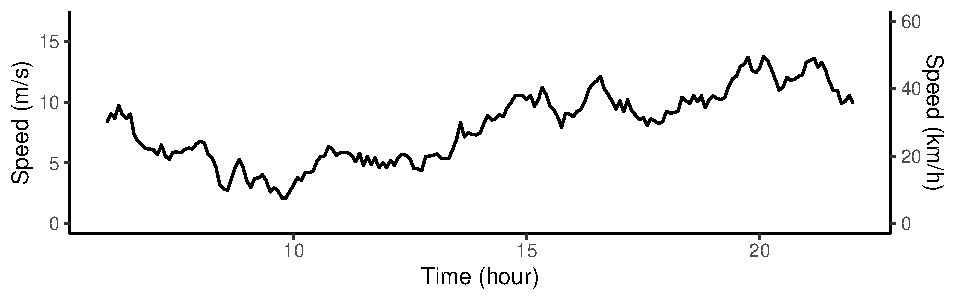
\includegraphics[width=0.8\textwidth]{figure/nw_sim_data-1} }\\
\subfloat[Actual bus speeds (averaged over road segment)\label{fig:nw_sim_data2}]{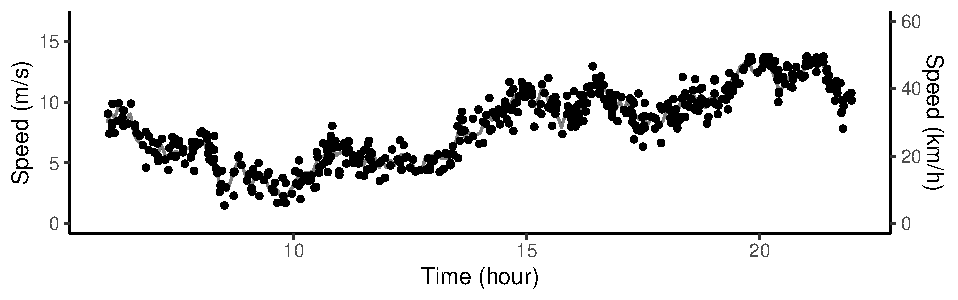
\includegraphics[width=0.8\textwidth]{figure/nw_sim_data-2} }\\
\subfloat[Observed average bus speeds, with vertial lines representing measurement error.\label{fig:nw_sim_data3}]{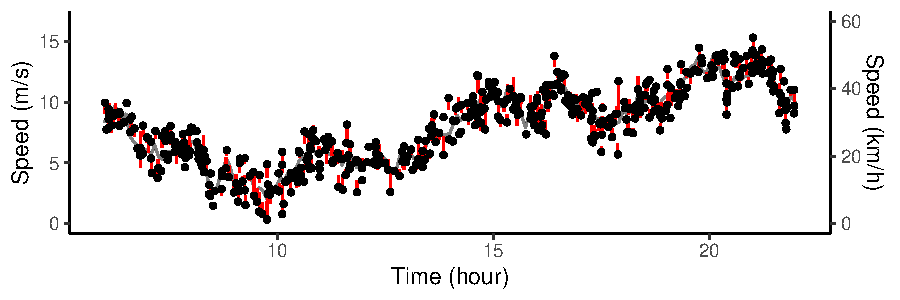
\includegraphics[width=0.8\textwidth]{figure/nw_sim_data-3} }\\

}

\caption[Simulated data showing average vehicle speed along a road]{Simulated data showing average vehicle speed along a road. The right hand axis is shown as a guide for readers not familiar with speeds measured in meters per second.}\label{fig:nw_sim_data}
\end{figure}


\end{knitrout}


Observed vehicle speeds for a real segment, displayed in \cref{fig:tt_figure}, shows some similarities to the simulated data, with one notable difference: the peak-hour spike. This spike is due, in part, to the location of the road, the Symonds Street overbridge\footnote{Anyone familiar with the area will understand the importance of this road}: there is often a (very long) queue of buses from many routes converging there on the central city. In this section, we use the simulated data to evaluate the model under ``nice'' conditions and then test it on this real data to see how well it copes with these types of phenomenon. The map in \cref{fig:nw_seg_maps} shows the location of this and other road segments.


\begin{knitrout}\small
\definecolor{shadecolor}{rgb}{0.969, 0.969, 0.969}\color{fgcolor}\begin{figure}

{\centering \subfloat[Travel time observations in seconds.\label{fig:tt_figure1}]{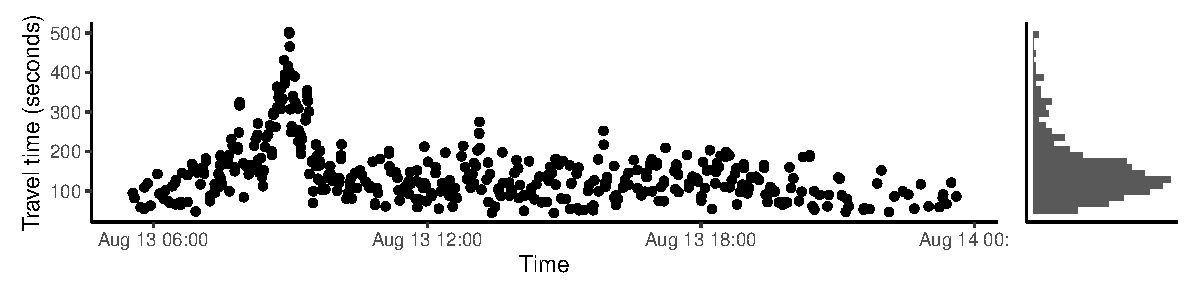
\includegraphics[width=\linewidth]{figure/tt_figure-1} }\\
\subfloat[Average speed in meters per second.\label{fig:tt_figure2}]{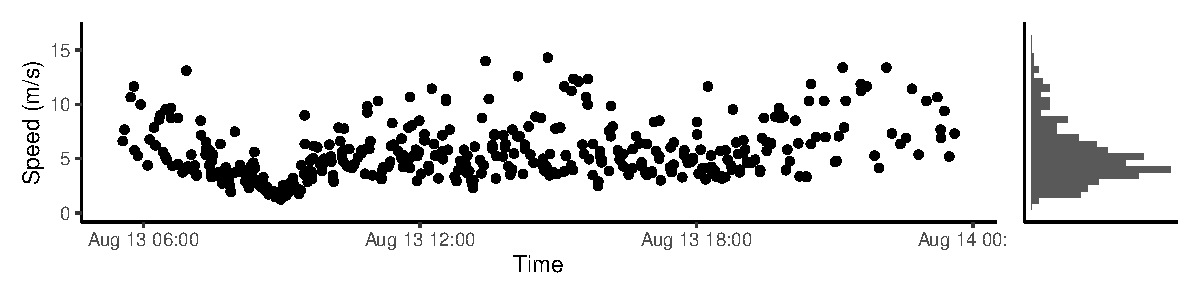
\includegraphics[width=\linewidth]{figure/tt_figure-2} }\\

}

\caption[Road state observations along a single road segment over time, with marginal historgrams on the right]{Road state observations along a single road segment over time, with marginal historgrams on the right.}\label{fig:tt_figure}
\end{figure}


\end{knitrout}
